\documentclass[11pt]{article}

% --- Style ---
\usepackage[nolinenumbers]{bioarxiv}

% --- Cross-reference main document ---
\usepackage{xr}
\externaldocument[main-]{main}

% --- Figures and tables ---
\usepackage{graphicx}
\graphicspath{{figures/}}
\usepackage{booktabs}

% --- Bibliography ---
\usepackage[numbers,sort&compress]{natbib}

% --- Subfigures ---
\usepackage{subcaption}

% --- Smart references (MUST load after hyperref, which is in bioarxiv.sty) ---
\usepackage{cleveref}

% --- S-prefixed counters ---
\renewcommand{\thefigure}{S\arabic{figure}}
\renewcommand{\thetable}{S\arabic{table}}
\renewcommand{\theequation}{S\arabic{equation}}
\renewcommand{\thesection}{S\arabic{section}}

% --- Override header for supplement ---
\fancyhead[L]{\small\color{preprint-gray}\textit{Supplementary Materials}}
\fancypagestyle{plain}{%
  \fancyhf{}%
  \fancyhf{}%
  \fancyhead[L]{\small\color{preprint-gray}\textit{Supplementary Materials}}%
  \fancyfoot[C]{\small\thepage}%
  \renewcommand{\headrulewidth}{0.4pt}%
}

% ====================================================================
\begin{document}

\begin{center}
  {\LARGE\bfseries Supplementary Materials}\\[1em]
  {\large Evo2 zero-shot variant effect prediction across 215,001 coding
         and non-coding variants in spaceflight radiation-response genes}\\[0.5em]
  {\normalsize JangKeun Kim, Christopher E. Mason}
\end{center}

\vspace{2em}

\tableofcontents

\clearpage

% ====================================================================
\section{Supplementary Methods}
\label{sec:supp_methods}

\subsection*{Genome and annotation versions}
All analyses used the GRCh38/hg38 reference genome (GCA\_000001405.15). Gene
coordinates, transcripts, and exon boundaries were extracted from NCBI RefSeq
annotations. ClinVar variant classifications (release 2024-12) were filtered to
$\geq$2-star review status. The gnomAD v4.1 constraint metrics were used for
gene-level loss-of-function intolerance scores.

\subsection*{Evo2 model and hardware}
Variant scoring used the Evo2 7-billion-parameter model~\cite{Evo2_2026},
trained on the OpenGenome2 dataset (9.3 trillion nucleotides). The model supports
context windows up to 1\,Mb; we used an 8,192\,\bp{} scoring window centred on
each variant (see main text \S2.1). All inference was performed on NVIDIA A40
(48\,GB VRAM) and A100 (40\,GB and 80\,GB VRAM) GPUs on the Cornell Cayuga HPC
cluster.

\subsection*{Variant scoring procedure}
For each variant, the reference and alternate alleles were embedded in the
genomic context. The model computed per-nucleotide log-likelihoods for both
sequences. The variant effect score ($\Delta$LL) was defined as the sum of
log-likelihood differences across all positions in the scoring window:
\begin{equation}
  \Delta\text{LL} = \sum_{i=1}^{W} \left[\log P(\text{alt}_i \mid \text{context}_\text{alt}) - \log P(\text{ref}_i \mid \text{context}_\text{ref})\right]
  \label{eq:delta_ll}
\end{equation}
where $W = 8{,}192$ is the window size. More negative $\Delta$LL values indicate
greater predicted deleteriousness. For indels, the window was adjusted to
accommodate the length difference while maintaining the same genomic centre.

\subsection*{DMS data processing}
Deep mutational scanning datasets were obtained from MaveDB~\cite{MaveDB_2019}:
BRCA1 (urn:mavedb:00000097-0-2; Findlay SGE~\cite{BRCA1_DMS_2018}),
TP53 (urn:mavedb:00000068-b-1; Giacomelli nutlin-3~\cite{TP53_DMS_2018}),
CHEK2 (urn:mavedb:00001203-a-1; McCarthy-Leo abundance~\cite{CHEK2_DMS_2024}).
DNMT3A paired DMS data were obtained from Garcia et al.~\cite{DNMT3A_DMS_2025}
(bioRxiv 10.1101/2025.09.24.678339). Library-relative positions were converted to
absolute genomic coordinates using verified offsets (Library 1: +655, Library 2:
+809, Library 3: +831). All DMS-to-genome mappings were validated by confirming
100\% reference allele match against GRCh38.

\subsection*{MPRA data processing}
TERT promoter MPRA data were obtained from MaveDB
(urn:mavedb:00000031-b-1; Kircher et al.~\cite{TERT_MPRA_2019}, GBM cell line).
Of 973 variants assayed, 777 mapped to the Evo2-scored region. Because TERT is
on the minus strand, forward-strand coordinates were used for all analyses, with
appropriate complement operations for variant alleles.

\subsection*{Bootstrap confidence intervals}
95\% confidence intervals for AUROCs were computed using stratified bootstrap
resampling (1,000 iterations), maintaining the pathogenic/benign ratio in each
resample.

\subsection*{DeLong test for AUROC comparison}
Pairwise AUROC differences between tools were assessed using the DeLong
test~\cite{DeLong_1988}, which accounts for the correlation between ROC curves
computed on overlapping variant sets. The Sun \& Xu (2014) fast algorithm was
used for variance estimation.

\subsection*{Transversion control analysis}
To test whether the elevated Evo2 scores for radiation-signature mutations
(C$>$A and G$>$T transversions) reflect radiation-specific chemistry rather than
general transversion bias, we compared $\Delta$LL distributions between
radiation-oxidative transversions and other transversions
(C$>$G, G$>$C, A$>$T, T$>$A, A$>$C, C$>$A excluded, G$>$T excluded, T$>$G)
using the Mann--Whitney $U$ test with rank-biserial correlation. $P$-values were
Bonferroni-corrected for 10 genes.

% ====================================================================
\clearpage
\section{Supplementary Figures}
\label{sec:supp_figs}

\begin{figure}[p]
  \centering
  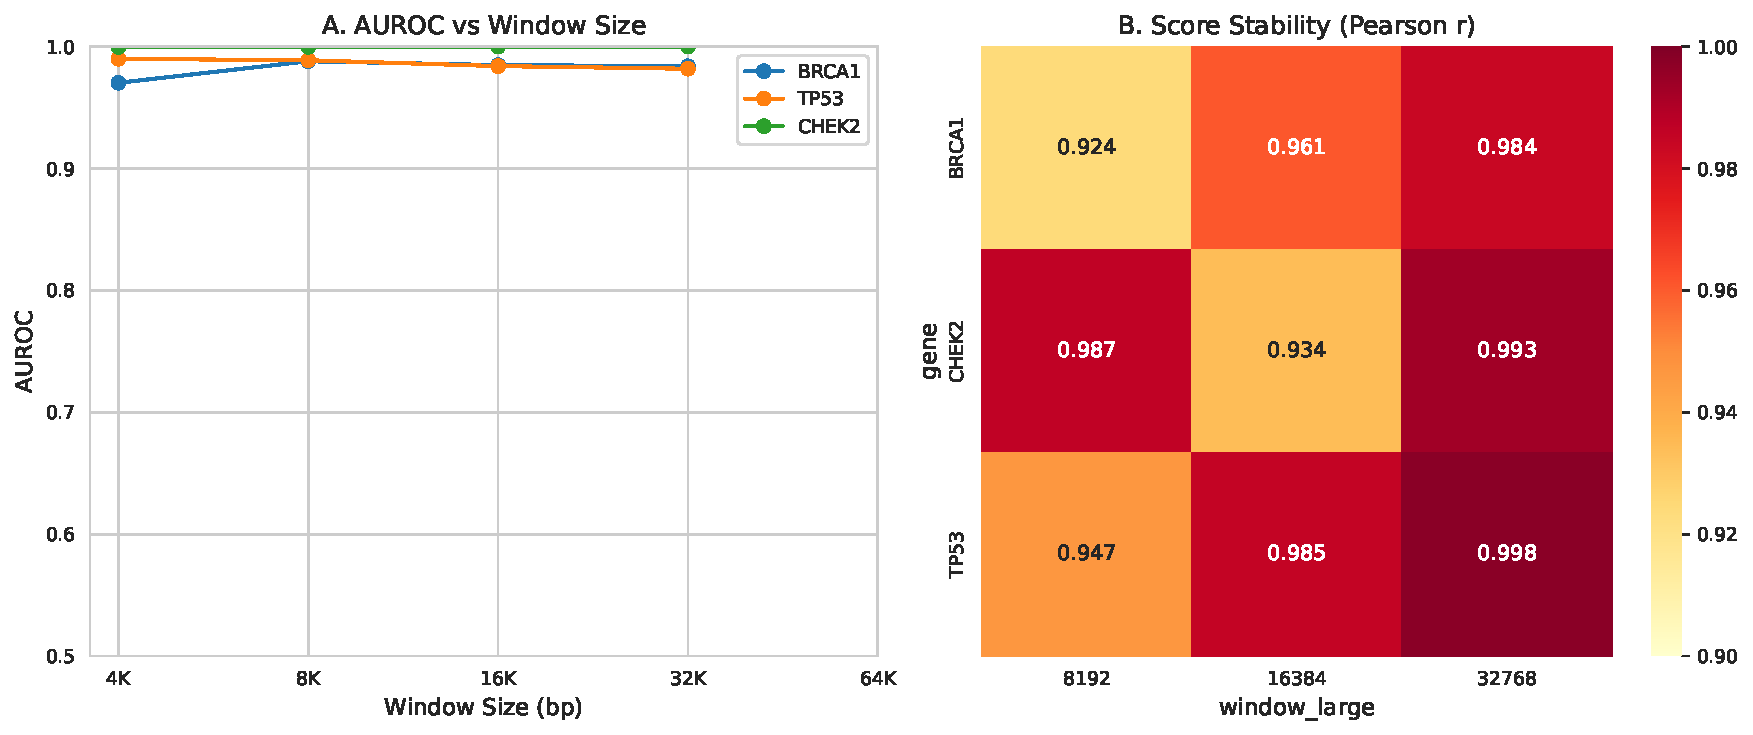
\includegraphics[width=\linewidth]{supp_s1_ablation}
  \caption{\textbf{Window size optimization.}
    ClinVar AUROC as a function of scoring window size (1024, 2048, 4096,
    8192\,\bp) for BRCA1, TP53, and CHEK2. The 8,192\,\bp{} window achieves
    the highest mean AUROC ($0.9921$) and was selected for all subsequent analyses.}
  \label{fig:supp_ablation}
\end{figure}

\begin{figure}[p]
  \centering
  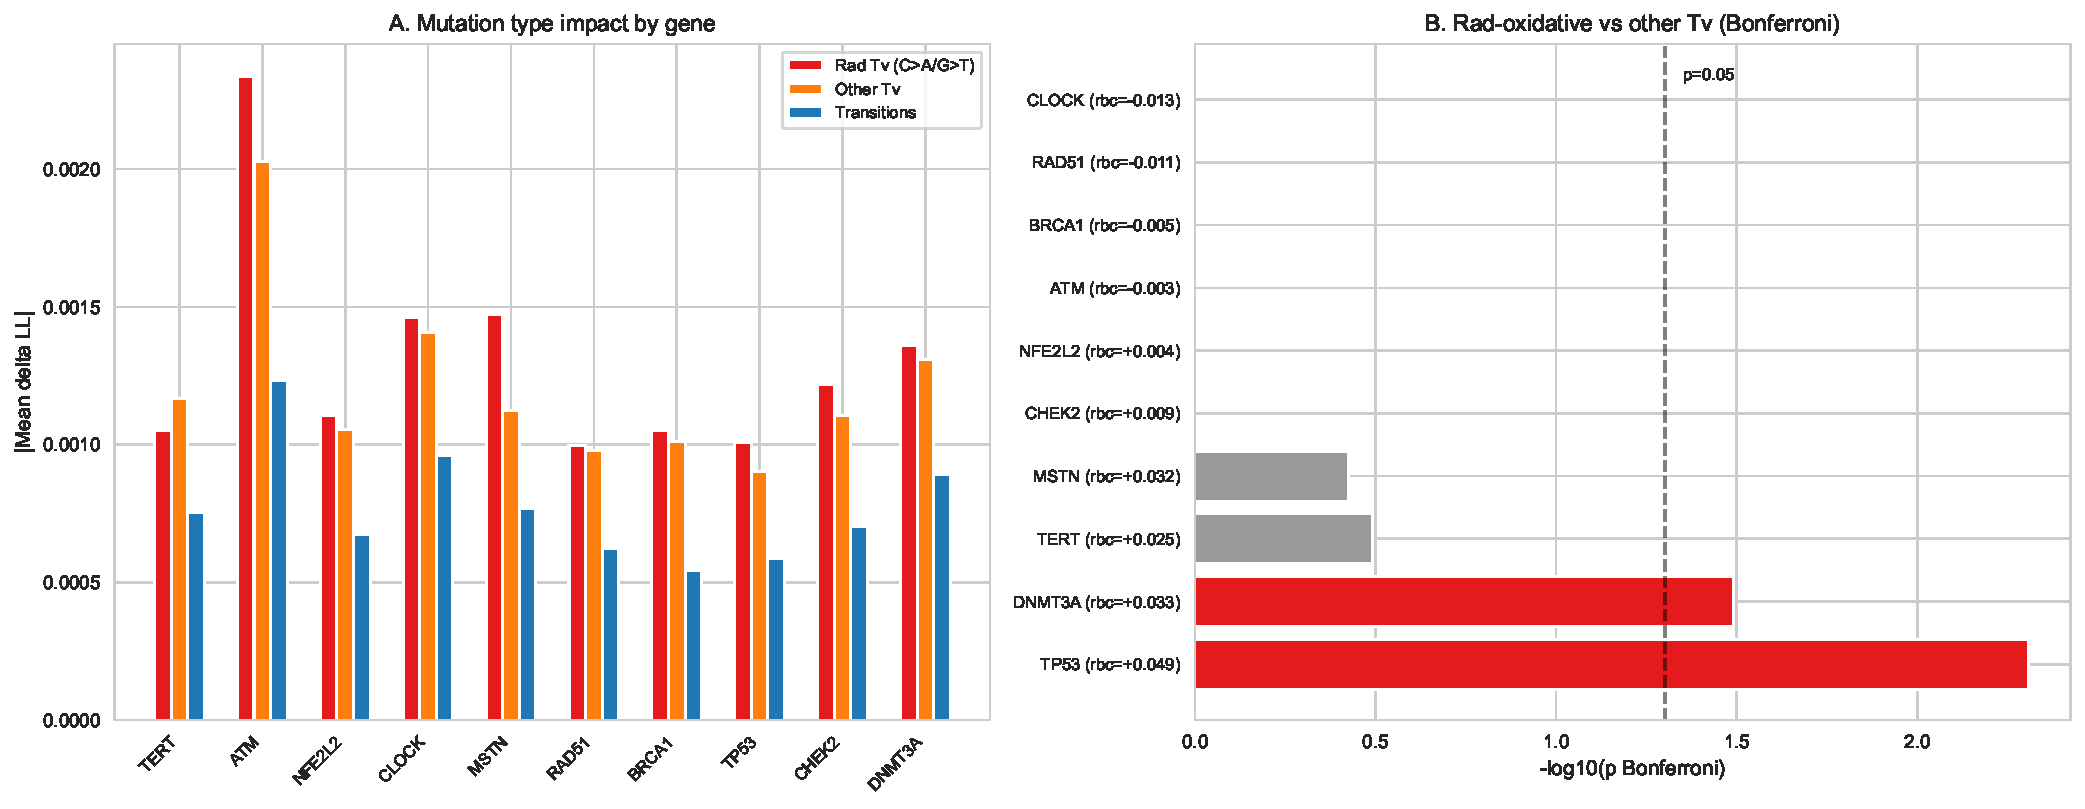
\includegraphics[width=\linewidth]{supp_s2_signatures}
  \caption{\textbf{Mutation signature analysis.}
    \textbf{(A)} Distribution of Evo2 $\Delta$LL by four-class mutation type
    (transition, transversion, frameshift, in-frame indel) for each gene;
    transversions score more deleterious than transitions in all ten genes
    ($p < 10^{-10}$).
    \textbf{(B)} Transversion control: radiation-oxidative (C$>$A/G$>$T) vs.\
    other transversions. After Bonferroni correction, only TP53 ($p = 0.005$,
    $r_{bc} = +0.049$) and DNMT3A ($p = 0.032$, $r_{bc} = +0.033$) show
    marginal radiation-specific signal; 8/10 genes are not significant.
    \textbf{(C)} Microhomology-mediated deletions show consistently elevated
    predicted deleteriousness across genes.}
  \label{fig:supp_signatures}
\end{figure}

\begin{figure}[p]
  \centering
  
\includegraphics[width=\linewidth]{supp_s3_indels}
  \caption{\textbf{Indel scoring detail.}
    Per-gene breakdown of frameshift vs.\ in-frame indel Evo2 $\Delta$LL
    distributions, with ClinVar P/LP vs.\ B/LB classification AUROCs for
    frameshift variants.}
  \label{fig:supp_indels}
\end{figure}

\begin{figure}[p]
  \centering
  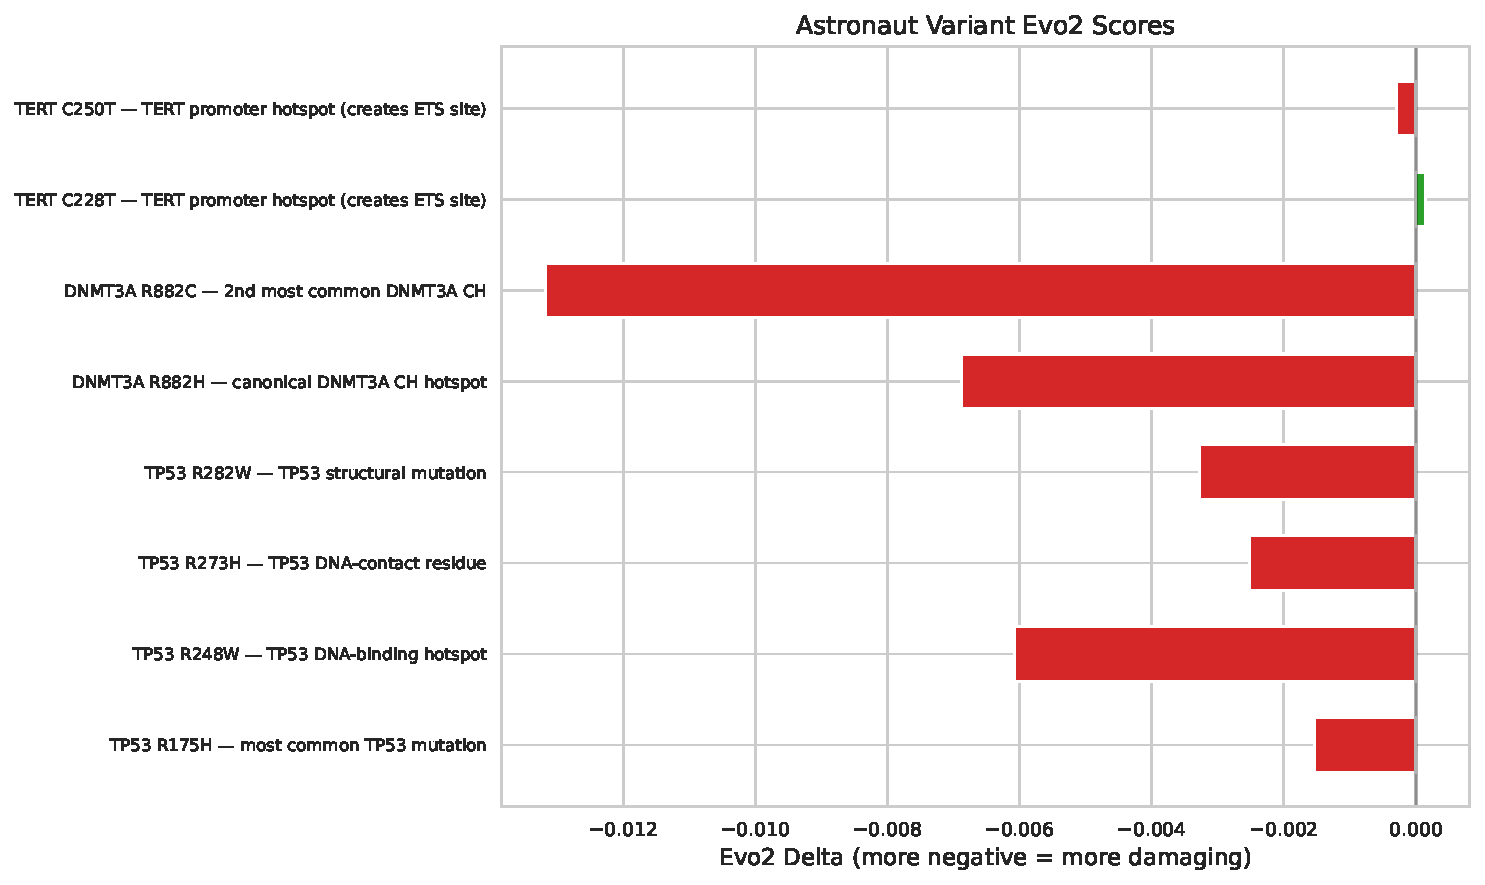
\includegraphics[width=\linewidth]{supp_s4_astronauts}
  \caption{\textbf{Astronaut variant case studies.}
    Eight variants detected in astronaut genomes~\cite{Rutter_2024}, scored
    by Evo2 with gene-level percentile rankings. Notable: DNMT3A R882C
    (97.2nd percentile, somatic hotspot), TP53 R248W (86.5th percentile),
    TERT C228T (4th percentile --- expected low score for gain-of-function
    promoter variant).}
  \label{fig:supp_astronauts}
\end{figure}

% ====================================================================
\clearpage
\section{Supplementary Tables}
\label{sec:supp_tables}

\begin{table}[h]
  \centering
  \caption{\textbf{Gene panel: coordinates, transcripts, and selection rationale.}
    All coordinates are GRCh38. Four control genes (BRCA1, TP53, CHEK2, DNMT3A) were
    selected for their extensive DMS/ClinVar annotation; six spaceflight-associated genes
    (TERT, ATM, NFE2L2, CLOCK, MSTN, RAD51) were selected based on radiation-response
    and spaceflight biology literature~\cite{Rutter_2024,daSilveira_2020}.}
  \label{tab:gene_panel}
  \small
  \begin{tabular}{lllrl}
    \toprule
    Gene & Chr & Coordinates & Variants & Category \\
    \midrule
    ATM     & 11 & 108,222,484--108,369,102 & 52,791 & DNA damage response \\
    BRCA1   & 17 & 43,044,295--43,125,483  & 36,901 & DNA damage response \\
    DNMT3A  & 2  & 25,227,855--25,342,590  & 19,693 & Epigenetic regulation \\
    CLOCK   & 4  & 56,294,068--56,413,912  & 18,369 & Circadian rhythm \\
    TERT    & 5  & 1,253,167--1,295,068    & 17,443 & Telomere maintenance \\
    CHEK2   & 22 & 28,687,743--28,742,422  & 16,098 & DNA damage response \\
    NFE2L2  & 2  & 177,230,308--177,264,876 & 15,230 & Oxidative stress \\
    TP53    & 17 & 7,661,779--7,687,550    & 14,240 & DNA damage response \\
    MSTN    & 2  & 190,055,700--190,062,718 & 12,383 & Muscle homeostasis \\
    RAD51   & 15 & 40,694,774--40,732,340  & 11,853 & DNA damage response \\
    \midrule
    \multicolumn{3}{l}{\textbf{Total}} & \textbf{215,001} & \\
    \bottomrule
  \end{tabular}
\end{table}

\begin{table}[h]
  \centering
  \caption{\textbf{DMS calibration: data sources and multi-tool Spearman correlations.}
    $|\rho|$ values are shown; sign convention: Evo2 $\Delta$LL is negative for damaging
    (positive $\rho$ = correct direction for BRCA1/CHEK2/DNMT3A; negative $\rho$ for TP53
    reflects LOF assay polarity where high DMS score = loss of function).
    AM = AlphaMissense; n.s.\ = $p > 0.05$.}
  \label{tab:dms_multitool}
  \small
  \begin{tabular}{lrrrrrr}
    \toprule
    Gene & $n$ & Evo2 & AM & CADD & REVEL & SpliceAI \\
    \midrule
    BRCA1  & 3,884 & 0.515 & 0.562 & 0.499 & 0.470 & 0.273 \\
    DNMT3A & 746   & 0.457 & 0.672 & 0.267 & 0.519 & 0.137 \\
    CHEK2  & 4,882 & 0.310 & 0.362 & 0.370 & 0.254 & 0.069 \\
    TP53   & 2,827 & 0.211 & 0.414 & 0.301 & 0.413 & n.s.  \\
    \bottomrule
  \end{tabular}
\end{table}

\begin{table}[h]
  \centering
  \caption{\textbf{ClinVar benchmarking: per-tool and matched-variant AUROCs with 95\% bootstrap CIs.}
    Per-tool AUROCs use all ClinVar variants scoreable by each tool independently.
    Matched AUROCs use the intersection of variants scored by all four tools
    (Evo2 $\cap$ CADD $\cap$ AM $\cap$ REVEL). --- indicates insufficient
    variants ($n < 10$).}
  \label{tab:clinvar_aurocs}
  \small
  \begin{tabular}{lrllll}
    \toprule
    Gene & $n$ (per-tool) & Evo2 & CADD & AM & REVEL \\
    \midrule
    \multicolumn{6}{l}{\textit{Per-tool AUROCs}} \\
    ATM    & 3,398 & 0.996 [0.993, 0.998] & 0.999 [0.998, 1.000] & 0.926 [0.870, 0.969] & --- \\
    BRCA1  & 2,676 & 0.988 [0.984, 0.992] & 0.995 [0.992, 0.997] & 0.960 [0.935, 0.980] & --- \\
    TP53   & 839   & 0.989 [0.983, 0.993] & 0.988 [0.979, 0.995] & 0.988 [0.978, 0.996] & --- \\
    CHEK2  & 689   & \textbf{1.000} [0.999, 1.000] & 0.999 [0.996, 1.000] & --- ($n=8$)  & --- \\
    DNMT3A & 159   & 0.996 [0.989, 1.000] & 1.000 [1.000, 1.000] & 1.000 [1.000, 1.000] & --- \\
    TERT   & 715   & 0.909 [0.832, 0.974] & 0.999 [0.997, 1.000] & 0.969 [0.893, 1.000] & --- \\
    \midrule
    \multicolumn{6}{l}{\textit{Matched-variant AUROCs (Evo2 $\cap$ CADD $\cap$ AM $\cap$ REVEL)}} \\
    ATM    & 86  & 0.864 & 0.940 & 0.924 & 0.941 \\
    BRCA1  & 335 & 0.932 & 0.957 & 0.960 & 0.916 \\
    TP53   & 271 & 0.894 & 0.920 & 0.988 & 0.967 \\
    DNMT3A & 18  & 0.847 & 1.000 & 1.000 & 0.972 \\
    TERT   & 22  & 0.866 & 0.991 & 0.969 & 0.991 \\
    CHEK2  & 8   & \multicolumn{4}{l}{--- (insufficient variants)} \\
    \bottomrule
  \end{tabular}
\end{table}

\begin{table}[h]
  \centering
  \caption{\textbf{Transversion control: radiation-oxidative vs.\ other transversions.}
    Mann--Whitney $U$ test comparing Evo2 $\Delta$LL distributions between
    C$>$A/G$>$T (radiation-oxidative) and other transversions. $r_{bc}$: rank-biserial
    correlation (positive = radiation more damaging). $P$-values are Bonferroni-corrected
    ($\times 10$).}
  \label{tab:transversion}
  \small
  \begin{tabular}{lrrrl}
    \toprule
    Gene & $p$ (raw) & $p$ (Bonferroni) & $r_{bc}$ & Significant? \\
    \midrule
    TP53   & 0.0005 & \textbf{0.005} & $+0.049$ & Borderline \\
    DNMT3A & 0.003  & \textbf{0.032} & $+0.033$ & Borderline \\
    TERT   & 0.032  & 0.322          & $+0.025$ & No \\
    MSTN   & 0.037  & 0.375          & $+0.032$ & No \\
    BRCA1  & 0.698  & 1.000          & $-0.005$ & No \\
    ATM    & 0.645  & 1.000          & $-0.003$ & No \\
    NFE2L2 & 0.381  & 1.000          & $+0.004$ & No \\
    CLOCK  & 0.839  & 1.000          & $-0.013$ & No \\
    RAD51  & 0.757  & 1.000          & $-0.011$ & No \\
    CHEK2  & 0.268  & 1.000          & $+0.009$ & No \\
    \bottomrule
  \end{tabular}
\end{table}

% --- Bibliography (shared with main) ---
\bibliographystyle{unsrtnat}
\bibliography{references}

\end{document}
